\documentclass[a4paper, 12pt,twoside]{book}

% set the paper size and the margins
\usepackage[top = 2cm, bottom = 2cm, left = 2cm, right = 3cm ]{geometry}
% set the header and the footnote
\usepackage{fancyhdr}
\pagestyle{fancy}
\fancyhf{}
\fancyhead[CE,CO]{Descriptive Statistics}
\fancyfoot[LE,RO]{\thepage}
% Supress the hyphenation
\hyphenation{thatshouldnot}
\usepackage{tablefootnote}
\usepackage{amsmath,amsfonts,amsthm}
\usepackage{multirow}
\usepackage{hhline}



\usepackage[]{graphicx}
\usepackage[]{color}
%% maxwidth is the original width if it is less than linewidth
%% otherwise use linewidth (to make sure the graphics do not exceed the margin)
\makeatletter
\def\maxwidth{ %
  \ifdim\Gin@nat@width>\linewidth
    \linewidth
  \else
    \Gin@nat@width
  \fi
}
\makeatother

\definecolor{fgcolor}{rgb}{0.345, 0.345, 0.345}
\newcommand{\hlnum}[1]{\textcolor[rgb]{0.686,0.059,0.569}{#1}}%
\newcommand{\hlstr}[1]{\textcolor[rgb]{0.192,0.494,0.8}{#1}}%
\newcommand{\hlcom}[1]{\textcolor[rgb]{0.678,0.584,0.686}{\textit{#1}}}%
\newcommand{\hlopt}[1]{\textcolor[rgb]{0,0,0}{#1}}%
\newcommand{\hlstd}[1]{\textcolor[rgb]{0.345,0.345,0.345}{#1}}%
\newcommand{\hlkwa}[1]{\textcolor[rgb]{0.161,0.373,0.58}{\textbf{#1}}}%
\newcommand{\hlkwb}[1]{\textcolor[rgb]{0.69,0.353,0.396}{#1}}%
\newcommand{\hlkwc}[1]{\textcolor[rgb]{0.333,0.667,0.333}{#1}}%
\newcommand{\hlkwd}[1]{\textcolor[rgb]{0.737,0.353,0.396}{\textbf{#1}}}%
\let\hlipl\hlkwb

\usepackage{framed}
\makeatletter
\newenvironment{kframe}{%
 \def\at@end@of@kframe{}%
 \ifinner\ifhmode%
  \def\at@end@of@kframe{\end{minipage}}%
  \begin{minipage}{\columnwidth}%
 \fi\fi%
 \def\FrameCommand##1{\hskip\@totalleftmargin \hskip-\fboxsep
 \colorbox{shadecolor}{##1}\hskip-\fboxsep
     % There is no \\@totalrightmargin, so:
     \hskip-\linewidth \hskip-\@totalleftmargin \hskip\columnwidth}%
 \MakeFramed {\advance\hsize-\width
   \@totalleftmargin\z@ \linewidth\hsize
   \@setminipage}}%
 {\par\unskip\endMakeFramed%
 \at@end@of@kframe}
\makeatother

\definecolor{shadecolor}{rgb}{.97, .97, .97}
\definecolor{messagecolor}{rgb}{0, 0, 0}
\definecolor{warningcolor}{rgb}{1, 0, 1}
\definecolor{errorcolor}{rgb}{1, 0, 0}
\newenvironment{knitrout}{}{} % an empty environment to be redefined in TeX

\usepackage{alltt}


% packages will be used by the 'kable' package
\usepackage{booktabs}
\usepackage{longtable}
\usepackage{array}
\usepackage{multirow}
\usepackage[table]{xcolor}
\usepackage{wrapfig}
\usepackage{float}
\usepackage{colortbl} 
\usepackage{pdflscape}
\usepackage{tabu}
\usepackage{threeparttable}
\usepackage{threeparttablex}
\usepackage[normalem]{ulem}
\usepackage{makecell}
\usepackage{xcolor}
\IfFileExists{upquote.sty}{\usepackage{upquote}}{}

% define a color for highlight
\definecolor{asparagus}{rgb}{0.53, 0.66, 0.42}
\definecolor{babypink}{rgb}{0.96, 0.76, 0.76}
\definecolor{champagne}{rgb}{0.97, 0.91, 0.81}
\definecolor{forestgreen}{rgb}{0.13, 0.55, 0.13}
\definecolor{dollarbill}{rgb}{0.52, 0.73, 0.4}


\begin{document}

\chapter{Descriptive statistics}
\thispagestyle{empty}
Statistics is a science of data. To study statistics, we have to describe data from some proper perspectives. Generally speaking, there are two ways to describe data, graphical description and numerical description. Those are what we are going to learn in this section.
\newpage

\begin{center}
\begin{knitrout}
\definecolor{shadecolor}{rgb}{0.969, 0.969, 0.969}\color{fgcolor}\rowcolors{2}{gray!6}{white}

\begin{table}[!h]
\caption{\label{ExampleData}Example Data\tablefootnote{MID is the scores in the midterm exam. FINAL is the scores in the final exam. BASKETBALL indicates whether a student plays basketball or not.}}
\centering
\scalebox{0.8}{
\begin{tabular}[t]{cccccc}
\hiderowcolors
\toprule
 NAME& CLASS & GENDER & MID & FINAL & BASKETBALL\\
\midrule
\showrowcolors
James & 23 & M & 74 & 86 & N\\
Andrew & 23 & M & 74 & 86 & Y\\
Jim & 23 & M & 23 & 47 & Y\\
Kim & 23 & M & 61 & 78 & Y\\
Mark & 23 & M & 97 & 98 & N\\
Owen & 23 & M & 73 & 85 & Y\\
Cook & 23 & M & 98 & 99 & Y\\
Albert & 23 & M & 81 & 90 & Y\\
Donald & 23 & M & 70 & 84 & N\\
Peter & 23 & M & 53 & 72 & Y\\
Vince & 23 & M & 68 & 82 & Y\\
Davis & 23 & M & 83 & 91 & Y\\
Alan & 23 & M & 82 & 90 & Y\\
Nick & 23 & M & 64 & 80 & N\\
Elina & 23 & F & 72 & 85 & N\\
Daisy & 23 & F & 68 & 82 & Y\\
Crystal & 23 & F & 53 & 72 & N\\
Karida & 23 & F & 66 & 81 & N\\
Linda & 23 & F & 83 & 91 & N\\
Dale & 23 & F & 70 & 83 & Y\\
Sandy & 23 & F & 56 & 74 & N\\
Emma & 23 & F & 65 & 80 & N\\
Angela & 23 & F & 72 & 85 & N\\
Katie & 23 & F & 84 & 91 & N\\
Eileen & 23 & F & 73 & 85 & N\\
Meggie & 23 & F & 68 & 82 & N\\
Jack & 24 & M & 45 & 67 & Y\\
Stan & 24 & M & 23 & 47 & Y\\
Ryan & 24 & M & 60 & 77 & Y\\
Murphy & 24 & M & 36 & 60 & N\\
Mike & 24 & M & 82 & 90 & Y\\
Antony & 24 & M & 18 & 42 & Y\\
Clare & 24 & M & 86 & 93 & Y\\
David & 24 & M & 83 & 91 & Y\\
Taylor & 24 & M & 69 & 83 & Y\\
Park & 24 & M & 78 & 88 & N\\
Gary & 24 & M & 51 & 71 & Y\\
Carson & 24 & M & 85 & 92 & Y\\
Elvis & 24 & M & 25 & 49 & Y\\
Kelly & 24 & F & 59 & 76 & N\\
Sara & 24 & F & 77 & 88 & N\\
Cherry & 24 & F & 61 & 78 & N\\
Lucy & 24 & F & 54 & 73 & Y\\
Hellen & 24 & F & 46 & 68 & N\\
Chloe & 24 & F & 95 & 97 & Y\\
Dorothy & 24 & F & 82 & 90 & N\\
Natalie & 24 & F & 73 & 85 & N\\
Vivien & 24 & F & 76 & 87 & N\\
Cathy & 24 & F & 70 & 84 & N\\
Carol & 24 & F & 55 & 74 & N\\
Bella & 24 & F & 96 & 98 & Y\\
Veronica & 24 & F & 60 & 77 & N\\
\bottomrule
\end{tabular}
}
\end{table}

\rowcolors{2}{white}{white}
\end{knitrout}
\end{center}
\section{Basic concepts}
\begin{itemize}
\item In  table \ref{ExampleData}, each student is an \textbf{individual}.
\item All students are described through perspectives of \textit{NAME, CLASS, GENDER, MID, FINAL,} and \textit{BASKETBALL}. Those different perspectives are called \textbf{variables}, for they may take different values for different students.
\item The values of \textit{MID} and \textit{FINAL} can be operated on like normal numbers, such as taking average, subtraction. Those variables are called 
\textbf{quantitative variables}.
\item The values of \textit{NAME, CLASS, GENDER} and \textit{BASKETBALL} only play the role of sorting individuals into different categories. Those variables are called \textbf{categorical variables}
\item The way a variable takes different values is called the \textbf{distribution} of this variable.
\item All the individuals we want to study is called the \textbf{population}.
\item A subset of the population is called a \textbf{sample}.

\colorbox{babypink}{Samples and populations are relative.} If you take all the Chinese people as the population, people in Shanghai is a sample. If you take all the people of the whole world as the population, then Chinese people is a sample.
\item The number of individuals in the sample is called the \textbf{sample size}.

\end{itemize}



\colorbox{babypink}{\parbox{15.2cm}{A variable takes values of numbers doesn't mean it is quantitative variable. Is variable \textit{CLASS} a quantitative or categorical variable?}}

\section{Some basic graphs}
\begin{itemize}
\item \textbf{Pie chart}
There are 25 girls and 27 boys in table \ref{ExampleData}. The pie chart of the  distribution of \textit{GENDER} is given by figure \ref{piechart}.
  \begin{center}
    \begin{figure}[!htb]
     \centering
    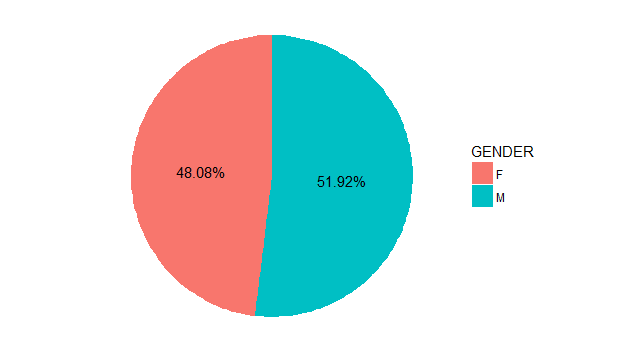
\includegraphics[scale=0.35]{PieChart.png}
    \caption{Pie chart of the distribution of the \textit{GENDER} }
    \label{piechart}
    \end{figure}  
\end{center} 

\item \textbf{Bar graph}

Similarly, we can draw bar graph to show the information about \textit{GENDER}
    \begin{figure}[H]
      \centering
        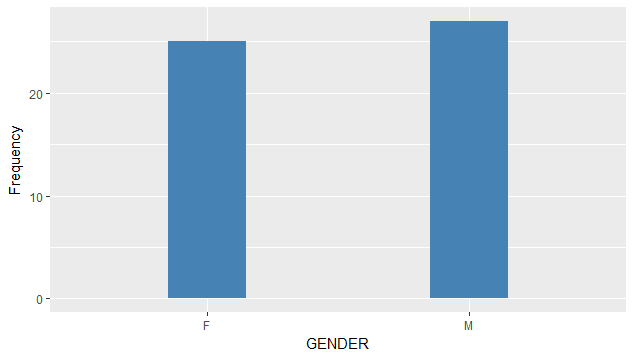
\includegraphics[scale=0.4]{Bargraph1.png}
        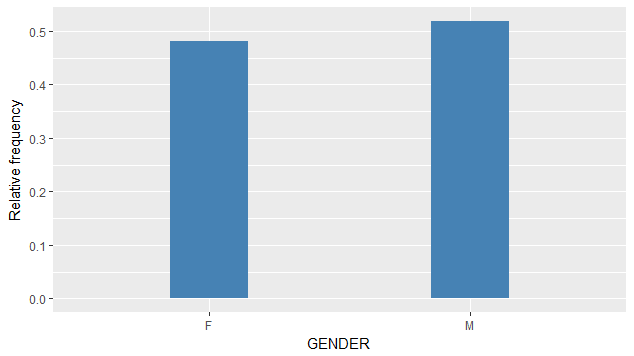
\includegraphics[scale=0.4]{Bargraph2.png}       
          \caption{Bar graphs with percentage and frequency as vertical axis} 
          \label{bargraph}
    \end{figure}    
 In figure \ref{bargraph}, the vertical axes are \textbf{frequency} and  \textbf{percentage} or (\textbf{relative frequency}) respectively. When the sample size is too big, it is better to use relative frequency as the vertical axis.
 
\colorbox{babypink}{\parbox{15.2cm}{Be sure to label the axes whenever a graph is drawn!}}

\item \textbf{Dotplot}
\begin{figure}[H]
\centering
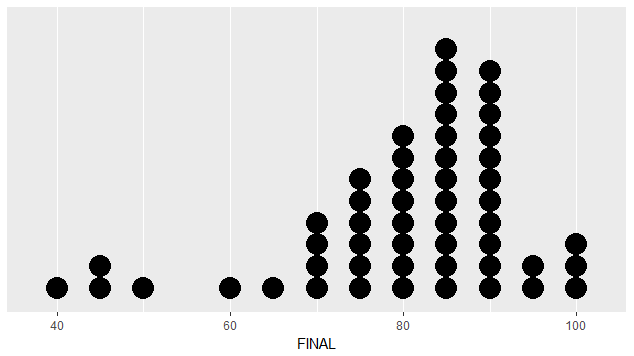
\includegraphics[scale=0.5]{Dotplot.png}
\caption{Dotplot of the distribution of the \textit{FINAL}}
\label{dotplot}
\end{figure}
In figure \ref{dotplot}, the \textbf{bin width} is 5. For example, there is only one score lies in the interval $(37.5, 42.5]$, which is "42" from the student whose name is "Antony", and the width of this interval is $42.5-37.5 = 5$, which is the bin width. Similarly, there are eight scores lies in the interval $(77.5, 82.5]$. 

\item \textbf{Histogram}

If the dots in dotplot is replaced by bars, the graph will be histogram, as shown in figure 

\begin{figure}[H]
\centering
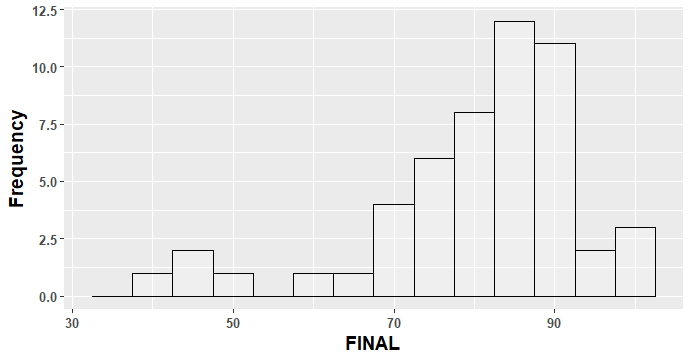
\includegraphics[scale=0.4]{Histogram1.png}
\caption{Histogram of the distribution of the \textit{FINAL}}
\label{HistogramFrequency}
\end{figure}
The vertical axis can be relative frequency as well.
\begin{figure}[H]
\centering
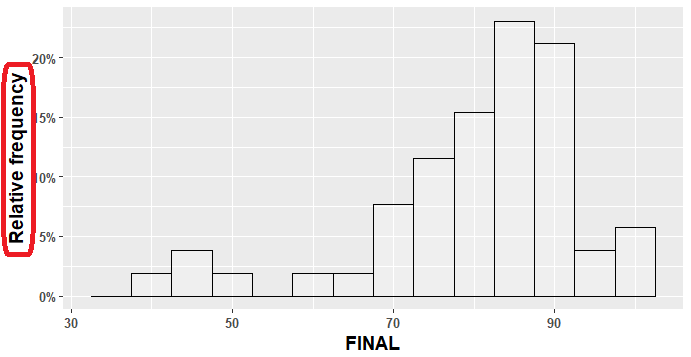
\includegraphics[scale=0.4]{Histogram2.png}
\caption{Histogram of with vertical axis \textbf{relative frequency}}
\label{HistogramRelativeFrequency}
\end{figure}

\colorbox{dollarbill}{\parbox{15.2cm}{What is the difference between histogram and bar graph?}}
\vspace{3cm}

\item \textbf{Density curve}

In figure \ref{HistogramRelativeFrequency}, we can tell the percentage of \textit{FINAL} $\leq 50$ is approximately $8\%$ by adding up the percentages of the first three columns. Here, the percentages are indicated by the height of the bars. (4 out of 52 students with \textit{FINAL} $\leq 50 $. They are 42, 47, 47, 49. )

Now, if we draw a histogram with bin width 1(figure \ref{HistogramBinWidth1}), then the percentage a bar can be calculated by
$$\textbf{percentage} = \textbf{bar height} = \textbf{bin width} * \textbf{bar height} = \textbf{area of the bar}.$$

\begin{figure}[H]
\centering
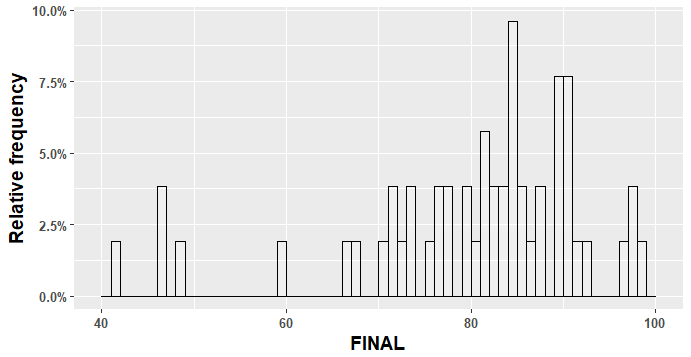
\includegraphics[scale=0.45]{Histogram3.png}
\caption{Histogram  with bin width 1}
\label{HistogramBinWidth1}
\end{figure}
If we want to calculate the percentage of the students with \textit{FINAL}$\leq 50$, we just add up the areas of the three bars to the left side of 50. 

\colorbox{dollarbill}{\parbox{15.2cm}{What is the total area of all bars in the histogram?}}
\vspace{1cm}

Take a step further. We want to draw a smooth curve such that the area to the left side of $\mathbf{x}$ gives the percentage of the number of individuals $\leq \mathbf{x}$.This type of graph is called \textbf{density curve}. The function of the density curve is called \textbf{probability density function(pdf)}.
\begin{figure}[H]
\centering
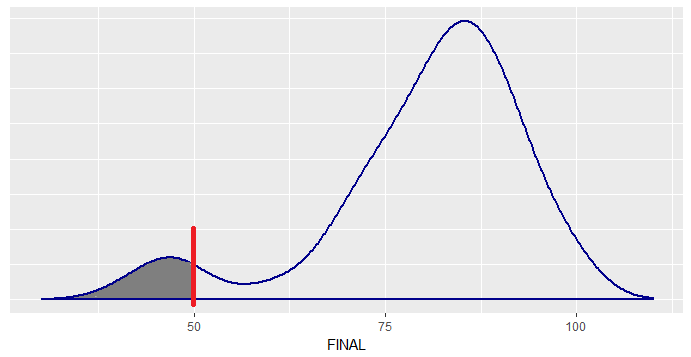
\includegraphics[scale=0.45]{DensityCurve.png}
\caption{Density curve of the distribution of the \textit{FINAL}}
\label{DensityCurve}
\end{figure}
Figure \ref{DensityCurve} is a density curve of the districution of the \textit{FINAL}, the shaded area gives the percentage of \textit{FINAL}$\leq 50$, which is approximately $8\%$.

\colorbox{babypink}{\parbox{15.2cm}{Sometimes the vertical axis may be suppressed, because it doesn't mean too much in this book.}}

\colorbox{dollarbill}{\parbox{15.2cm}{What is the total area under the density curve?}}
\vspace{1cm}
\item \textbf{Cumulative relative frequency curve}

In figure \ref{DensityCurve}, for each value of $\mathbf{x}$ there is an area to the left side of this value. Therefore we can get a function $F$,such that 
$$F(x) = \textbf{Area to the left of } \mathbf{x}.$$
If we draw a smooth graph of $F(x)$, it will be like figure \ref{CumulativeRFCurve}. This curve is called the \textbf{cumulative relative frequency curve.} Function $F(x)$ is called \textbf{cumulative density function(cdf)}.

\begin{figure}[H]
\centering
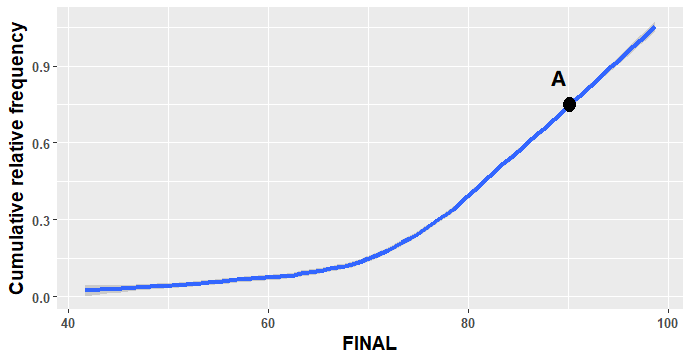
\includegraphics[scale=0.5]{CumulativeRFCurve.png}
\caption{Cumulative relative frequency curve of \textit{FINAL}}
\label{CumulativeRFCurve}
\end{figure}

\colorbox{dollarbill}{\parbox{15.2cm}{How to interpret point \textbf{A} in figure \ref{CumulativeRFCurve}?}}

\colorbox{dollarbill}{\parbox{15.2cm}{What is the theoretical relation between figure \ref{CumulativeRFCurve} and figure \ref{DensityCurve}?}}

\end{itemize}
\vspace{3cm}

\section{Some terms to describe graphs}
\begin{itemize}
\item \textbf{Shape}
\begin{figure}[H]
\centering
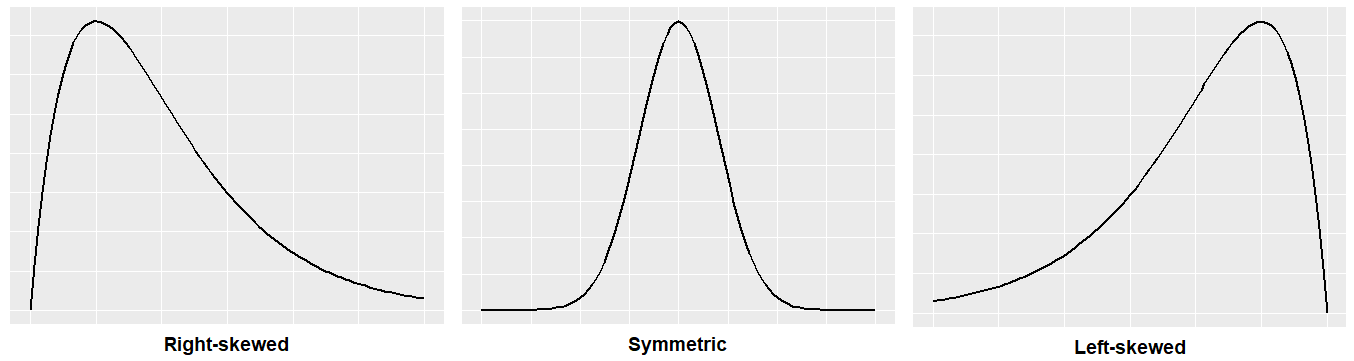
\includegraphics[scale=0.35]{Skewness.png}
\caption{Shapes of distributions}
\label{Skewness}
\end{figure}
As shown in figure \ref{Skewness}, the shapes of the distributions are \textbf{right-skewed, symmetric} and \textbf{left-skewed} respectively.

\begin{figure}[H]
\centering
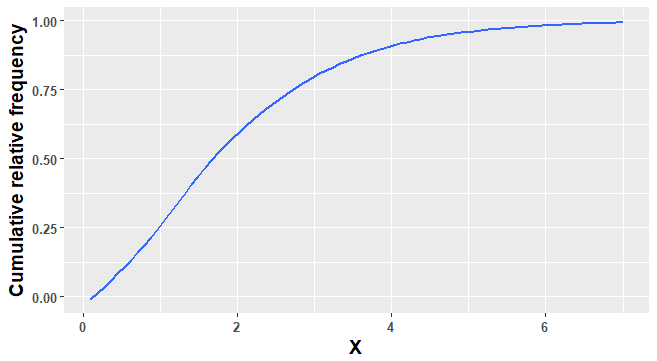
\includegraphics[scale=0.4]{CumulativeSkew.png}
\caption{A cumulative relative frequency curve}
\label{CumulativeSkew}
\end{figure}
\colorbox{dollarbill}{\parbox{15.2cm}{Can you tell whether the distribution in figure \ref{CumulativeSkew} is right-skewed, left-skewed or symmetric?}}
\vspace{3cm}
\item \textbf{Clusters and gaps}
\begin{figure}[H]
\centering
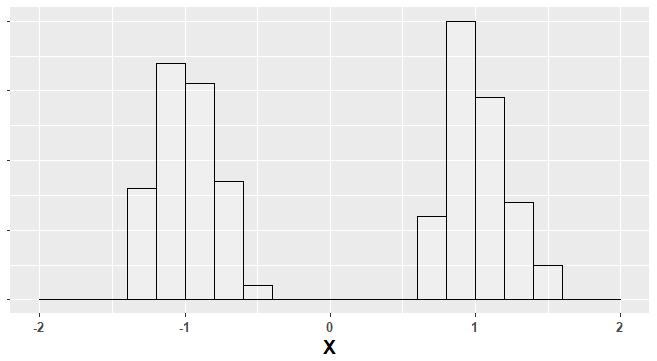
\includegraphics[scale=0.4]{TwoClusters.png}
\caption{Two clusters and a gap}
\label{TwoClusters}
\end{figure}
As show in figure \ref{TwoClusters}, we say the distribution has two \textbf{clusters(modes)} with a \textbf{gap}.

\item \textbf{Outliers}
\begin{figure}[H]
\centering
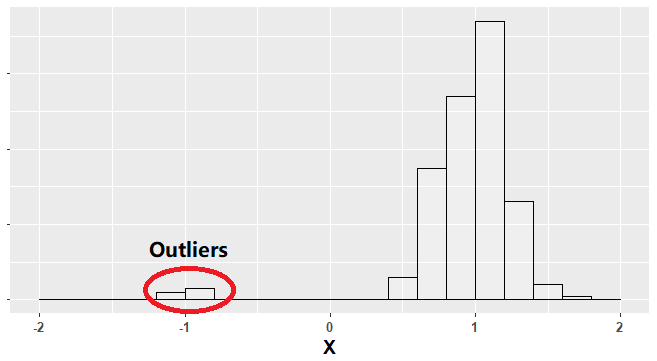
\includegraphics[scale=0.4]{Outliers.png}
\caption{Outliers}
\label{Outliers}
\end{figure}

If some values have striking departures from the pattern of the majority, those values are called \textbf{outliers}.
 
\colorbox{babypink}{\parbox{15.2cm}{Outliers need special attention, for they may be generated by mistakes or some other mechanisms that are not considered.}}
\end{itemize}
\section{Summarizing distributions}
\begin{itemize}
\item \textbf{Center}

There are different ways to describe the center of a distribution. Here we only consider two primary ways of denoting the center:\textbf{median} and \textbf{mean}.

\begin{itemize}
 \item \textbf{Median}
 
 Arrange the data in increasing or decreasing order, median is the middle one or the average of the middle two. 
 
 \item \textbf{Mean}
 
 For data set $\{x_1, x_2, \cdots, x_n\}$, the mean $\bar{x}$ is given by 
 $$\bar{x} = \frac{x_1+x_2+\cdots+x_n}{n}
           = \frac{\sum_{i=1}^{n}x_i}{n} $$
\end{itemize}

\colorbox{babypink}{Sometime the notation of the mean is $\mu$.} $\mu$ is used for population mean, $\bar{x}$ is for sample mean. For example, we draw a sample of 100 students from a high school, and the mean weight of those 100 students is 60kg. We use  the notation $\bar{x}$, because the mean weight 60kg comes from the sample of 100 students. If the mean weight of all the students in this high school is 60kg, we use the notation $\mu$. The formulas for $\mu$ and $\bar{x}$  are the same.

\colorbox{babypink}{When to use mean and when to use median? }Let's take a look at a simple example. Say, we have a set of data $\{1, 2, 3, 4, 5\}$. Both the mean and the median are 3. If 5 is recorded as 500 by accident. Now, the mean is 102, while the median is still the same. That is to say, the median is not easily influenced by the extreme values. If a value is not easily influenced by extreme values, it is \textbf{resistant}.

The relationship of the mean and median can be shown by figure \ref{MeanMedian}.
\begin{figure}[H]
\centering
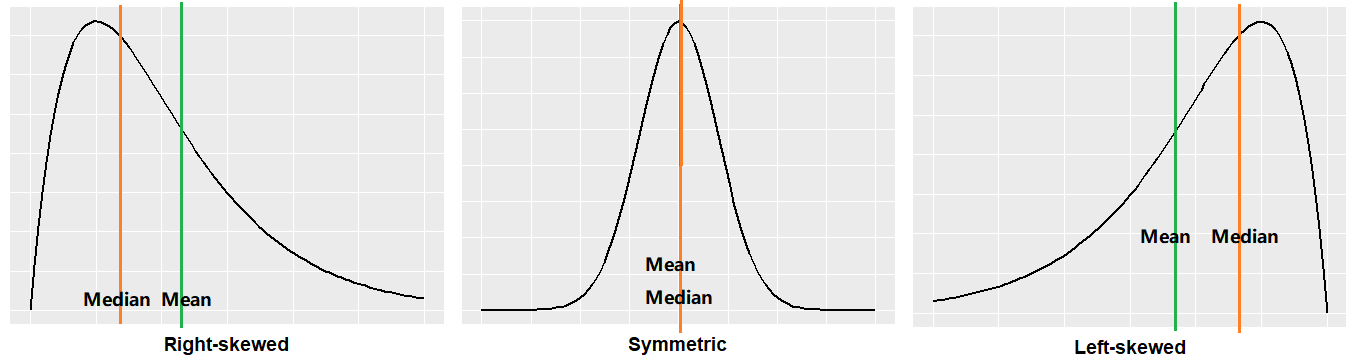
\includegraphics[scale=0.35]{MeanMedian.png}
\caption{The relationship between mean and median}
\label{MeanMedian}
\end{figure}

Generally speaking, if the distribution is symmetric, $\textbf{mean} = \textbf{median}$; if the distribution is right-skewed, $\textbf{mean} > \textbf{median}$; if the distribution is left-skewed, $\textbf{mean} < \textbf{median}$. A simple explanation comes as: if the distribution is right-skewed, there are more extreme values to the right side. While the mean is not so resistant as median, it can be more easily dragged to the right than the median. Thus $\textbf{mean} > \textbf{median}$.

\colorbox{babypink}{\parbox{15.2cm}{Therefore, if the distribution is strongly skewed, it is better to use the \textbf{median} to describe the center of the distribution.}}

\colorbox{dollarbill}{\parbox{15.2cm}{Is mean or median a better description of the center of the distribution of personal incomes?}}
\vspace{3cm}
\item \textbf{Spread}

Spread is to measure the variability or the dispersion of the data.
\begin{itemize}
\item \textbf{Range}

The difference between the maximun and the minimum, $$\textbf{range} = \textbf{maximun} - \textbf{minimum}$$

\item \textbf{Interquartile range(IQR)}

\textbf{First quartile($Q_1$)} is the value with one quarter of the data less than(or equal) to it. For data $\{1,2,3,4,5,6,7,8\}$, 2 is the first quartile.

\textbf{Third quartile($Q_1$)} is the value with $3/4$ of the data less than(or equal) to it. For data $\{1,2,3,4,5,6,7,8\}$, 6 is the third quartile.

Interquartile range is given by $$\textbf{IQR} = \mathbf{Q_3} - \mathbf{Q_1}.$$
For data $\{1,2,3,4,5,6,7,8\}$, the interquartile range $\textbf{IQR} = 6-2=4$

\item \textbf{Variance(Var)}

$$\textbf{Population variance}\;\;\;Var=\sigma^2=\frac{\sum_{i=1}^{n}(x_i-\mu)^2}{n}.$$

$$\textbf{Sample variance}\;\;\;Var=s_x^2=\frac{\sum_{i=1}^{n}(x_i-\bar{x})^2}{n}.$$

Variance gives the average square of the difference between the mean and data.

\item \textbf{Standard deviation}

$$\textbf{Population standard deviation}\hspace{0.5cm}\sigma=\sqrt[]{\frac{\sum_{i=1}^{n}(x_i-\mu)^2}{n}}.$$
$$\textbf{Sample standard deviation}\hspace{0.5cm}\bar{x}=\sqrt[]{\frac{\sum_{i=1}^{n}(x_i-\bar{x})^2}{n}}.$$

\colorbox{babypink}{Standard deviation gives the average distance of the data from the mean.}
\begin{itemize}
\item \colorbox{dollarbill}{\parbox{13.2cm}{Calculate the mean and standard deviation of sample data $\{1, 2, 3\}$ by hand}}
\vspace{1cm}
\item \colorbox{dollarbill}{\parbox{13.2cm}{Calculate the mean and standard deviation of the \textit{FINAL} of students in class 23 by calculator.}}
\vspace{1cm}
\end{itemize}


\end{itemize}
\item \textbf{Location}
\begin{itemize}
\item \textbf{Percentile}

$n^{th}$ percentile is the value with n percent of the data smaller or equal to it. For data $\{1, 2, 3, 4, 5, 6, 7, 8, 9, 10\}$, 1 is the $10^{th}$ percentile, 6 is the $60^{th}$ percentile.
\colorbox{dollarbill}{What percentiles are $Q_1$, median and $Q_3$?}
\vspace{1cm}

\begin{itemize}

\item \textbf{Five number summary}
There are five important locations for a given set of data, they are \textbf{min}, $\mathbf{Q_1}$, \textbf{median}, $\mathbf{Q_3}$ and \textbf{max}. They are called a \textbf{five number summary}. The following is a five number summary of the \textit{FINAL}.
\begin{center}
\definecolor{shadecolor}{rgb}{0.969, 0.969, 0.969}\color{fgcolor}\begin{kframe}
\begin{verbatim}
##    Min.     Q1.   Median     Q3.    Max. 
##   42.00   75.50   83.50    90.00   99.00
\end{verbatim}
\end{kframe}
\end{center}
\vspace{0.6cm}
\item \textbf{1.5 IQR rule} gives a simple rule to tell whether a value is an outlier or not. 
$$x \notin [Q_1-1.5 \times IQR,\; Q_3+1.5 \times IQR] \implies \text{x is an outlier}.$$
\colorbox{dollarbill}{Find out the outliers of the \textit{FINAL} by the 1.5 IQR rule.}
\vspace{1cm}
\item \textbf{Boxplot}
\begin{figure}[H]
\centering
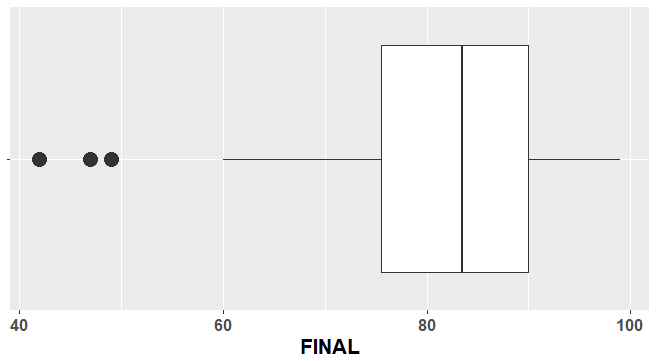
\includegraphics[scale=0.5]{Boxplot.png}
\caption{The boxplot of the \textit{FINAL}}
\label{Boxplot}
\end{figure}
In figure \ref{Boxplot}, the three dots are outliers, the left vertical line of the box indicates the value of the $Q_1$, the middle vertical line indicates the median and the right vertical line indicates the $Q_3$.

\end{itemize}

\item \textbf{z-score}

For a value $x$, its z-score is given by $$z=\frac{x-\mu}{\sigma}.$$
\colorbox{babypink}{The z-score  gives the distance from the mean in terms of standard deviation.}

\end{itemize}

\colorbox{dollarbill}{Calculate and interpret the z-score of the \textit{FINAL} of Vince.}

\colorbox{dollarbill}{Calculate the percentile of the \textit{FINAL} of Vince.}

\colorbox{dollarbill}{Of the measurements of the spread, which are more resistant and which are not?}

\item \textbf{Data transformation}

Suppose we have a sample data set $\mathbf{X} = \{x_1, x_2, \cdots, x_n\}$ with mean $\bar{x}$ and standard deviation $s_x$ . 

\begin{itemize}
\item Add a constant $c$ to the data
$$\mathbf{X}+c = \{x_1+c, x_2+c, \cdots, x_n+c\}.$$
\begin{equation*}
\begin{split}
\text{The mean of}\;\mathbf{X}+c &= \frac{(x_1+c)+(x_2+c)+\cdots+(x_n+c)}{n}\\
&= \frac{x_1+x_2+\cdots+x_n}{n}+ c\\
&= \bar{x} + c.
\end{split}
\end{equation*}
\colorbox{babypink}{The mean is added by the same constant c.}
\begin{equation*}
\begin{split}
\text{The standard deviation of}\;\mathbf{X}+c &= \sqrt{\frac{\sum_{i=1}^n[(x_i+c)-(\bar{x}+c)]^2}{n}}\\
&= \sqrt{\frac{\sum_{i=1}^n(x_i-\bar{x})^2}{n}}\\
&= s_x.
\end{split}
\end{equation*}
\colorbox{babypink}{The standard deviation doesn't change.}

\colorbox{dollarbill}{What about the \textbf{IQR} and percentiles if the data is added by a constant c.}

\item Multiply the data by constant $a$
$$a\mathbf{X} = \{ax_1, ax_2, \cdots, ax_n\}.$$
\begin{equation*}
\begin{split}
\text{The mean of}\;\mathbf{aX} &= \frac{(ax_1)+(ax_2)+\cdots+(ax_n)}{n}\\
&= a\frac{x_1+x_2+\cdots+x_n}{n}\\
&= a\bar{x}.
\end{split}
\end{equation*}
\colorbox{babypink}{The mean is multiplied by the same constant a.}
\begin{equation*}
\begin{split}
\text{The standard deviation of}\;a\mathbf{X}&= \sqrt{\frac{\sum_{i=1}^n(ax_i-a\bar{x})^2}{n}}\\
&= |a|\sqrt{\frac{\sum_{i=1}^n(x_i-\bar{x})^2}{n}}\\
&= |a|s_x.
\end{split}
\end{equation*}
\colorbox{babypink}{The standard deivation is multiplied by the absolute value of constant a.}
\end{itemize}
\colorbox{dollarbill}{Calculate the mean and standard deviation of the z-scores for any give data set.}
\end{itemize}
\section{Comparing distributions}
\begin{itemize}
\item \textbf{Perspectives to describe a distribution}

When you are asked to describe the distribution give by a graph, you are supposed to describe the \textbf{shape, center} and \textbf{spread}. If there are \textbf{outliers, more than one clusters} and \textbf{gaps}, you are suppose to enunciate them.
\vspace{0.6cm}

For example, by referring to figure \ref{Boxplot}, we say the distribution of the \textit{FINAL} is roughly symmetric, with median around 84, and IQR about 16, and there are 3 outliers.

\item \textbf{Graphs for comparing distributions}

\begin{figure}[H]
\centering
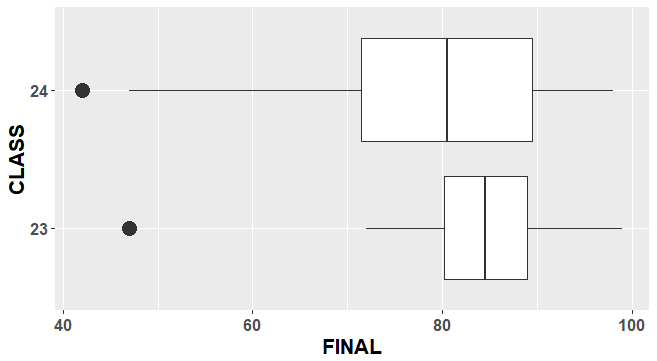
\includegraphics[scale=0.5]{BxoplotComparison.png}
\caption{Distributions of the \textit{FINAL} of \textit{CLASS} 23 and \textit{CLASS} 24}
\label{BxoplotComparison}
\end{figure}

\begin{figure}[H]
\centering
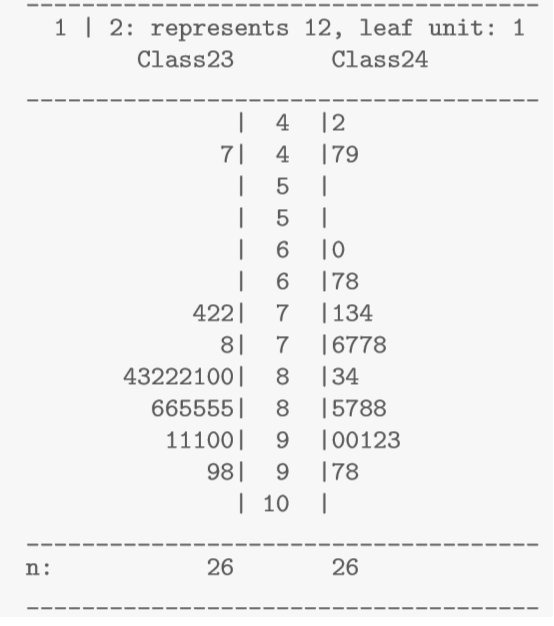
\includegraphics[scale=0.5]{BackToBackSplittingStemPlot.png}
\caption{Back-to-back stem plot with splitting stems}
\label{BackToBackSplittingStemPlot}
\end{figure}
There are many graphs to compare distributions. Figure \ref{BxoplotComparison} and figure \ref{BackToBackSplittingStemPlot} are about the distributions of the \textit{FINAL} of \textit{CLASS} 23 and \textit{CLASS} 24.

\item \textbf{Compare two distributions}

The distributions are compared through the same perspectives as when we describe the distributions. They are \textbf{shape, center} and \textbf{spread}, and \textbf{outliers, clusters} and \textbf{gaps} if necessary.
\vspace{0.6cm}

The terms to describe the shape are \textbf{right-skewed, symmetric} and \textbf{left-skewed}.

The terms to describe center are \textbf{mean} and \textbf{median}. Choose a appropriate one.

The terms to describe the spread are \textbf{range, IQR} and \textbf{standard deviation}. Choose a  appropriate one.
 

\vspace{0.6cm}
For example, if figure \ref{BxoplotComparison} is given. We can say:

 Both of the distributions are approximately symmetric. 
 
 The median of the \textit{FINAL} of \textit{CLASS} 24 is approximately 80, less than the median of the \textit{FINAL} of \textit{CLASS} 23, which is approximately 85.
 
 Then IQR of \textit{CLASS} 24 is approximately 20, larger than the IQR of \textit{CLASS} 23, which is about 10. Thus the \textit{FINAL} of \textit{CLASS} 24 is more widely spread than that of \textit{CLASS} 23 in the angle of IQR.
 
 Both of the distributions have an outlier to the lower end.
 
\colorbox{babypink}{Distribution comparison or distribution description problem always show up in AP exam.} 
\end{itemize}
\section{The relation between two variables}
\begin{itemize}
\item \textbf{Two categorical variables}
By reading table \ref{ExampleData}, we may suspect that the is a relation between categorical variable \textit{BASKETALL} and \textit{GENDER}. Maybe boys are more likely to play basketball than girls. How can we describe the relation between  \textit{BASKETALL} and \textit{GENDER}?
\begin{itemize}
\item \textbf{Two-way table}
\begin{table}[H]
\begin{center}
 \begin{tabular}{c|cccc}
\hline
\multicolumn{2}{c}{}&\multicolumn{2}{c}{BASKETBALL}&\multirow{2}{*}{Total}\\
\hhline{~~--~}
\multicolumn{2}{c}{}&\multicolumn{1}{c}{Yes}&\multicolumn{1}{c}{No}&\\
\multirow{2}{*}{GENDER}&Male&$21$&$6$&$27$\\
&Female&$5$&$20$&$25$\\
\multicolumn{2}{c}{Total}&$26$&$26$&$52$\\
\hline
 \end{tabular}
\caption{Two-way table of Gender $\times$ Basketball}
\label{Two-way table}
\end{center}
\end{table}
Table \ref{Two-way table} gives a simple description about the relation between \textit{BASKETALL} and \textit{GENDER}.
\begin{itemize}
 \item \textbf{Conditional distribution}
 \vspace{0.6cm}
 
 The \textbf{conditional distribution} of a categorical variable is defined as the distribution of this variable while the value of the other variable is fixed.
 \vspace{0.6cm}
 
 \begin{table}[H]
 \hspace{3cm}
 \begin{tabular}{ccc}
  \vspace{0.2cm}
 \textit{BASKETBALL}&Percentage of Male&Percentage of Female\\
 \hline
 
 \vspace{0.2cm}
 Yes&$\frac{21}{26} \approx 81\%$&$\frac{5}{26} \approx 19\%$\\
 \vspace{0.2cm}
  No&$\frac{6}{26} \approx 23\%$&$\frac{20}{26} \approx 77\%$\\
 \hline 
 \end{tabular}
 \caption{Conditional distribution}
 \label{ConditionalDistribution}
 \end{table}
 
Table \ref{ConditionalDistribution} gives the conditional distribution of \textit{GENDER} conditioned on different different values of \textit{BASKETBALL}. For example, the conditional distribution of \textit{GENDER} among those who play basketball is that: about $81\%$ of them are boys, $19\%$ are girls.
\vspace{0.6cm} 

If a student plays basketball, this students is more likely to be a boy than a girl. Clearly, there is some association between \textit{GENDER} and \textit{BASKETBALL}.
\vspace{0.6cm} 

\item \textbf{Association}
\vspace{0.6cm}

If the conditional distributions of a variable are different while conditioned on different values of the other variable, we say there is an \textbf{association} between those variables. Otherwise, they   are \textbf{independent}.
\vspace{0.6cm}

The conditional distributions of \textit{GENDER} are different conditioned on different values(Yes, No) of \textit{BASKETBALL}. Therefore, there is an association between \textit{GENDER} and \textit{BASKETBALL}.
\vspace{0.6cm}

\item \textbf{Marginal distribution}
\vspace{0.6cm}

If we consider the distribution of \textit{GENDER} regardless of the \textit{BASKETBALL}, we just look at the data at the right margin of tabel \ref{Two-way table}.
$$\text{Percentage of girls:}\hspace{0.3cm}\frac{25}{52} = 48\%,\hspace{0.6cm}\text{Percentage of boys:} \hspace{0.3cm} \frac{27}{52} = 52\%$$
Similarly, we can find out the distribution of \textit{BASKETBALL} regardless of the \textit{GENDER} by looking at the data at the bottom margin of tabel \ref{Two-way table}.
\vspace{0.6cm}

All the distributions are \textbf{marginal distribuions}, for we only consider the data at the margin of the two-way table.

\colorbox{dollarbill}{\parbox{13.2cm}{Is it true that if two variables have no association(independent), the marginal distributions and the conditional distributions are the same?}}
\end{itemize}
\vspace{0.6cm}
\item \textbf{Side-by-side bar graph}
\vspace{0.6cm}

\textbf{Side-by-side bar graph} is a graph to show the relation between two categorical variables.


\end{itemize}
\end{itemize}
\end{document}